\documentclass{standalone}
\usepackage{tikz}
\usetikzlibrary{patterns, positioning}


\begin{document}
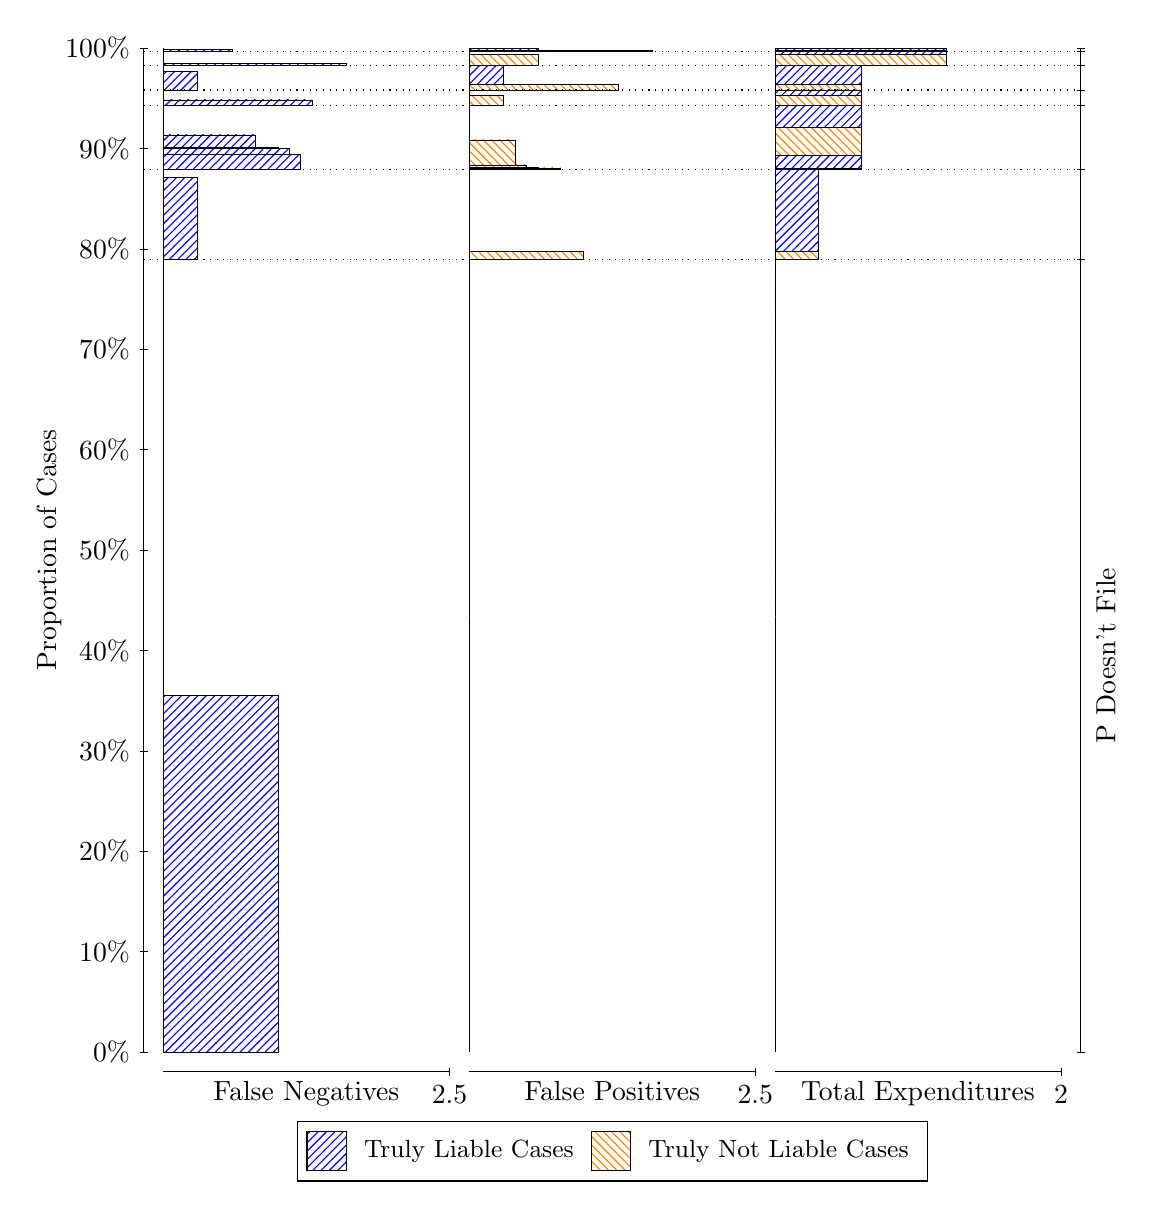
\begin{tikzpicture}
\draw[black, very thin] (1.5,1.75) -- (1.5,14.5);
\node[rotate=90, text=black, anchor=center] at (0.3, 8.125) {Proportion of Cases};
\draw[black, very thin] (1.45,1.75) -- (1.55,1.75);
\node[text=black, anchor=east] at (1.45, 1.75) {0\%};
\draw[black, very thin] (1.45,3.025) -- (1.55,3.025);
\node[text=black, anchor=east] at (1.45, 3.025) {10\%};
\draw[black, very thin] (1.45,4.3) -- (1.55,4.3);
\node[text=black, anchor=east] at (1.45, 4.3) {20\%};
\draw[black, very thin] (1.45,5.575) -- (1.55,5.575);
\node[text=black, anchor=east] at (1.45, 5.575) {30\%};
\draw[black, very thin] (1.45,6.85) -- (1.55,6.85);
\node[text=black, anchor=east] at (1.45, 6.85) {40\%};
\draw[black, very thin] (1.45,8.125) -- (1.55,8.125);
\node[text=black, anchor=east] at (1.45, 8.125) {50\%};
\draw[black, very thin] (1.45,9.4) -- (1.55,9.4);
\node[text=black, anchor=east] at (1.45, 9.4) {60\%};
\draw[black, very thin] (1.45,10.675) -- (1.55,10.675);
\node[text=black, anchor=east] at (1.45, 10.675) {70\%};
\draw[black, very thin] (1.45,11.95) -- (1.55,11.95);
\node[text=black, anchor=east] at (1.45, 11.95) {80\%};
\draw[black, very thin] (1.45,13.225) -- (1.55,13.225);
\node[text=black, anchor=east] at (1.45, 13.225) {90\%};
\draw[black, very thin] (1.45,14.5) -- (1.55,14.5);
\node[text=black, anchor=east] at (1.45, 14.5) {100\%};

\draw[black, very thin] (13.4,1.75) -- (13.4,14.5);
\draw[black, very thin] (13.35,1.75) -- (13.45,1.75);
\node[anchor=west] at (13.35, 1.75) {};
\draw[black, very thin] (13.35,11.813) -- (13.45,11.813);
\node[anchor=west] at (13.35, 11.813) {};
\draw[black, very thin] (13.35,12.962) -- (13.45,12.962);
\node[anchor=west] at (13.35, 12.962) {};
\draw[black, very thin] (13.35,13.768) -- (13.45,13.768);
\node[anchor=west] at (13.35, 13.768) {};
\draw[black, very thin] (13.35,13.967) -- (13.45,13.967);
\node[anchor=west] at (13.35, 13.967) {};
\draw[black, very thin] (13.35,14.276) -- (13.45,14.276);
\node[anchor=west] at (13.35, 14.276) {};
\draw[black, very thin] (13.35,14.453) -- (13.45,14.453);
\node[anchor=west] at (13.35, 14.453) {};
\draw[black, very thin] (13.35,14.5) -- (13.45,14.5);
\node[anchor=west] at (13.35, 14.5) {};

\draw[black, very thin, pattern color=blue, pattern=north east lines] (1.75,1.75) rectangle (3.2033,6.2807);
\draw[black, very thin, pattern color=orange, pattern=north west lines] (1.75,6.2807) rectangle (1.75,11.813);
\draw[black, very thin, pattern color=blue, pattern=north east lines] (1.75,11.813) rectangle (2.186,12.854);
\draw[black, very thin, pattern color=orange, pattern=north west lines] (1.75,12.854) rectangle (1.75,12.962);
\draw[black, very thin, pattern color=blue, pattern=north east lines] (1.75,12.962) rectangle (3.494,13.148);
\draw[black, very thin, pattern color=blue, pattern=north east lines] (1.75,13.148) rectangle (3.3487,13.229);
\draw[black, very thin, pattern color=blue, pattern=north east lines] (1.75,13.229) rectangle (3.2033,13.239);
\draw[black, very thin, pattern color=blue, pattern=north east lines] (1.75,13.239) rectangle (2.9127,13.396);
\draw[black, very thin, pattern color=orange, pattern=north west lines] (1.75,13.396) rectangle (1.75,13.768);
\draw[black, very thin, pattern color=blue, pattern=north east lines] (1.75,13.768) rectangle (3.6393,13.841);
\draw[black, very thin, pattern color=orange, pattern=north west lines] (1.75,13.841) rectangle (1.75,13.967);
\draw[black, very thin, pattern color=blue, pattern=north east lines] (1.75,13.967) rectangle (2.186,14.204);
\draw[black, very thin, pattern color=orange, pattern=north west lines] (1.75,14.204) rectangle (1.75,14.276);
\draw[black, very thin, pattern color=blue, pattern=north east lines] (1.75,14.276) rectangle (4.0753,14.308);
\draw[black, very thin, pattern color=orange, pattern=north west lines] (1.75,14.308) rectangle (1.75,14.453);
\draw[black, very thin, pattern color=blue, pattern=north east lines] (1.75,14.453) rectangle (2.622,14.481);
\draw[black, very thin, pattern color=orange, pattern=north west lines] (1.75,14.481) rectangle (1.75,14.5);
\draw[black, very thin, pattern color=orange, pattern=north west lines] (5.6333,1.75) rectangle (5.6333,7.2825);
\draw[black, very thin, pattern color=blue, pattern=north east lines] (5.6333,7.2825) rectangle (5.6333,11.813);
\draw[black, very thin, pattern color=orange, pattern=north west lines] (5.6333,11.813) rectangle (7.0867,11.921);
\draw[black, very thin, pattern color=blue, pattern=north east lines] (5.6333,11.921) rectangle (5.6333,12.962);
\draw[black, very thin, pattern color=orange, pattern=north west lines] (5.6333,12.962) rectangle (6.796,12.978);
\draw[black, very thin, pattern color=orange, pattern=north west lines] (5.6333,12.978) rectangle (6.5053,12.982);
\draw[black, very thin, pattern color=orange, pattern=north west lines] (5.6333,12.982) rectangle (6.36,13.016);
\draw[black, very thin, pattern color=orange, pattern=north west lines] (5.6333,13.016) rectangle (6.2147,13.334);
\draw[black, very thin, pattern color=blue, pattern=north east lines] (5.6333,13.334) rectangle (5.6333,13.768);
\draw[black, very thin, pattern color=orange, pattern=north west lines] (5.6333,13.768) rectangle (6.0693,13.894);
\draw[black, very thin, pattern color=blue, pattern=north east lines] (5.6333,13.894) rectangle (5.6333,13.967);
\draw[black, very thin, pattern color=orange, pattern=north west lines] (5.6333,13.967) rectangle (7.5227,14.039);
\draw[black, very thin, pattern color=blue, pattern=north east lines] (5.6333,14.039) rectangle (6.0693,14.276);
\draw[black, very thin, pattern color=orange, pattern=north west lines] (5.6333,14.276) rectangle (6.5053,14.421);
\draw[black, very thin, pattern color=blue, pattern=north east lines] (5.6333,14.421) rectangle (5.6333,14.453);
\draw[black, very thin, pattern color=orange, pattern=north west lines] (5.6333,14.453) rectangle (7.9587,14.472);
\draw[black, very thin, pattern color=blue, pattern=north east lines] (5.6333,14.472) rectangle (6.5053,14.5);
\draw[black, very thin, pattern color=orange, pattern=north west lines] (9.5167,1.75) rectangle (9.5167,7.2825);
\draw[black, very thin, pattern color=blue, pattern=north east lines] (9.5167,7.2825) rectangle (9.5167,11.813);
\draw[black, very thin, pattern color=orange, pattern=north west lines] (9.5167,11.813) rectangle (10.062,11.921);
\draw[black, very thin, pattern color=blue, pattern=north east lines] (9.5167,11.921) rectangle (10.062,12.962);
\draw[black, very thin, pattern color=orange, pattern=north west lines] (9.5167,12.962) rectangle (10.607,12.978);
\draw[black, very thin, pattern color=blue, pattern=north east lines] (9.5167,12.978) rectangle (10.607,13.135);
\draw[black, very thin, pattern color=orange, pattern=north west lines] (9.5167,13.135) rectangle (10.607,13.491);
\draw[black, very thin, pattern color=blue, pattern=north east lines] (9.5167,13.491) rectangle (10.607,13.768);
\draw[black, very thin, pattern color=orange, pattern=north west lines] (9.5167,13.768) rectangle (10.607,13.894);
\draw[black, very thin, pattern color=blue, pattern=north east lines] (9.5167,13.894) rectangle (10.607,13.967);
\draw[black, very thin, pattern color=orange, pattern=north west lines] (9.5167,13.967) rectangle (10.607,14.039);
\draw[black, very thin, pattern color=blue, pattern=north east lines] (9.5167,14.039) rectangle (10.607,14.276);
\draw[black, very thin, pattern color=orange, pattern=north west lines] (9.5167,14.276) rectangle (11.697,14.421);
\draw[black, very thin, pattern color=blue, pattern=north east lines] (9.5167,14.421) rectangle (11.697,14.453);
\draw[black, very thin, pattern color=orange, pattern=north west lines] (9.5167,14.453) rectangle (11.697,14.472);
\draw[black, very thin, pattern color=blue, pattern=north east lines] (9.5167,14.472) rectangle (11.697,14.5);
\draw[black, dotted] (1.5,11.813) -- (13.4,11.813);
\draw[black, dotted] (1.5,12.962) -- (13.4,12.962);
\draw[black, dotted] (1.5,13.768) -- (13.4,13.768);
\draw[black, dotted] (1.5,13.967) -- (13.4,13.967);
\draw[black, dotted] (1.5,14.276) -- (13.4,14.276);
\draw[black, dotted] (1.5,14.453) -- (13.4,14.453);
\draw[black, very thin] (1.75,1.5) -- (5.3833,1.5);
\node[text=black, anchor=north] at (3.5667, 1.5) {False Negatives};
\draw[black, very thin] (5.3833,1.45) -- (5.3833,1.55);
\node[text=black, anchor=north] at (5.3833, 1.45) {2.5};

\draw[black, very thin] (5.6333,1.5) -- (9.2667,1.5);
\node[text=black, anchor=north] at (7.45, 1.5) {False Positives};
\draw[black, very thin] (9.2667,1.45) -- (9.2667,1.55);
\node[text=black, anchor=north] at (9.2667, 1.45) {2.5};

\draw[black, very thin] (9.5167,1.5) -- (13.15,1.5);
\node[text=black, anchor=north] at (11.333, 1.5) {Total Expenditures};
\draw[black, very thin] (13.15,1.45) -- (13.15,1.55);
\node[text=black, anchor=north] at (13.15, 1.45) {2};

\node[text=black, centered, rotate=90] at (13.72, 6.7816) {P Doesn't File};







\draw (7.449999999999999,1.5) node[draw=none] (baseCoordinate) {};
\begin{scope}[align=center]
        \matrix[scale=0.5, draw=black, below=0.5cm of baseCoordinate, nodes={draw}, column sep=0.1cm]{
            \node[rectangle, draw, minimum width=0.5cm, minimum height=0.5cm, pattern color=blue, pattern=north east lines] {}; &
            \node[draw=none, font=\small, text=black] (B) {Truly Liable Cases}; &
            \node[rectangle, draw, minimum width=0.5cm, minimum height=0.5cm, pattern color=orange, pattern=north west lines] {}; &
            \node[draw=none, font=\small, text=black] (B) {Truly Not Liable Cases}; \\
            };
\end{scope}

\end{tikzpicture}
\end{document}